% arara: pdflatex: { shell: true, interaction: nonstopmode }
% arara: bibtex
% arara: makeglossaries
% arara: makeindex
% arara: pdflatex: { shell: true, interaction: nonstopmode }
% arara: pdflatex: { shell: true, interaction: nonstopmode }
\documentclass[11pt, a4paper, oneside, twocolumn]{report}
% .  ___   ___        ___  ___  ___   ___  ___  ___   ___              ___         ___   ___   ___ 
% . |   |=|_.'   .'|=|_.' `._|=|   |=|_.' `._|=|   |=|_.'   .'|   .'| |   |   .'|=|_.'  |   |=|_.' 
% . `.  |      .'  |  ___      |   |           |   |      .'  | .'  |\|   | .'  |___    `.  |      
% .   `.|=|`.  |   |=|_.'      |   |           |   |      |   | |   | |   | |   |`._|=.   `.|=|`.  
% .  ___  |  `.|   |  ___      `.  |           `.  |      |   | |   | |  .' `.  |  __||  ___  |  `.
% .  `._|=|___||___|=|_.'        `.|             `.|      |___| |___| |.'     `.|=|_.''  `._|=|___|
% .                                                                                                
%% packages --------------------------------------------------------------------
\usepackage{hyphenations} % thats my own hyphenation list
% \usepackage[english]{babel}
\usepackage[font={it}]{caption}
\usepackage[noend]{algpseudocode}
\usepackage[chapter]{mytodo} % thats my own todo package based on easy-todo
\usepackage{
  amsmath,
  amssymb,
  graphicx,
  hhline,
  hyphenat,
  ifdraft,
  listings,
  makeidx,
  pdfpages,
  pgfplots,
  siunitx,
  subcaption,
  tabularx,
  tikzinput,
  xcolor}
\usepackage[nottoc]{tocbibind} % hide toc itself from toc
\usepackage[hidelinks]{hyperref} % always load last!
\usepackage[acronym,nomain,toc]{glossaries} % always load after hyperref!
%% settings --------------------------------------------------------------------
\pgfplotsset{%
  width  = \textwidth,
  height = \textwidth,
  compat = 1.17,
  colormap name = viridis,
  cycle list name = exotic,
  table/search path={data},
} % TikZ doesnt know the twocolumn thing
\usetikzlibrary{external}
\usetikzlibrary{calc}
\tikzexternalize[optimize=true,prefix=tikz/] % externalize tikz, much faster, many conflicts!
\setcounter{secnumdepth}{2} % set level of depth for numbering
\graphicspath{{figures/}}
%% settings for listings
\lstset{
  basicstyle=\small,               % or \small or \footnotesize etc.
  backgroundcolor=\color{white},   % choose the background color; you must add \usepackage{color} or \usepackage{xcolor}; should come as last argument
  breaklines=true,                 % sets automatic line breaking
  captionpos=b,                    % sets the caption-position to bottom
  deletekeywords={...},            % if you want to delete keywords from the given language
  escapeinside={\%*}{*)},          % if you want to add LaTeX within your code
  firstnumber=1,                   % start line enumeration with line 1
  keepspaces=true,                 % keeps spaces in text, useful for keeping indentation of code (possibly needs columns=flexible)
  morekeywords={
  *,
  double,
  false,
  ifftshift,
   numel,
  true,
  .},            % if you want to add more keywords to the set
  numbers=left,                    % where to put the line-numbers; possible values are (none, left, right)
  numbersep=5pt,                   % how far the line-numbers are from the code
  numberstyle=\tiny\color{gray}, % the style that is used for the line-numbers
  rulecolor=\color{black},         % if not set, the frame-color may be changed on line-breaks within not-black text (e.g. comments (green here))
  showspaces=false,                % show spaces everywhere adding particular underscores; it overrides 'showstringspaces'
  showstringspaces=false,          % underline spaces within strings only
  showtabs=false,                  % show tabs within strings adding particular underscores
  stepnumber=1,                    % the step between two line-numbers. If it's 1, each line will be numbered
  tabsize=2,	                   % sets default tabsize to 2 spaces
  %title=\lstname                   % show the filename of files included with \lstinputlisting; also try caption instead of title
  %frame = single,
}
 % a lot of listing options
\renewcommand{\arraystretch}{1.2} % streches row heigth in arrays (and tables)
\DeclareSIUnit\molar{\mole\per\cubic\deci\metre}
\DeclareSIUnit\Molar{\textsc{m}}
%% makros ----------------------------------------------------------------------
\renewcommand{\b}{\textbf}
\renewcommand{\u}{\underline}
\renewcommand{\tt}{\texttt}
\renewcommand{\t}{\todo}
\newcommand{\e}{\emph}
\newcommand{\n}{\textnormal}
\newcommand{\m}{\mathrm}
\newcommand{\x}[1]{#1\index{#1}}
% .  ___  ___   ___        ___  ___   ___                   ___ 
% . `._|=|   |=|_.'   .'| `._|=|   |=|_.'   .'|        .'|=|_.' 
% .      |   |      .'  |      |   |      .'  |      .'  |  ___ 
% .      |   |      |   |      |   |      |   |      |   |=|_.' 
% .      `.  |      |   |      `.  |      |   |  ___ |   |  ___ 
% .        `.|      |___|        `.|      |___|=|_.' |___|=|_.' 
% .                                                            
\begin{document}
\begin{titlepage}
  \onecolumn
  \centering
  \large
  a\\
  \vspace{.5cm}
  {\Large \textsc{ Projektarbeit / Student Project}}\\
  \vspace{1cm}
  {\Huge \textsc{ Dual Channel Single Molecule Localisation Microscopy}}\\
  \vspace{1cm}
  concluded at the\\
  \vspace{.5cm}
  {\Large \textsc{Technische Universit\"at (Tu) Wien}}\\
  \vspace{.5cm}
  advised by\\
  \vspace{.5cm}
  {\Large \textsc{Lukas Velas}}\\
  \vspace{.5cm}
  of\\
  \vspace{.5cm}
  {\Large \textsc{Moritz Siegel}}\\
  \vfill
  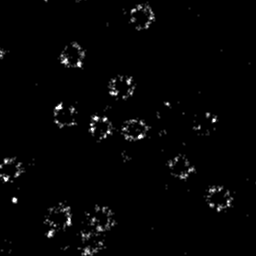
\includegraphics[scale=.5]{npc/npc256.png}\\
  \vfill
  Vienna\\
  \today\\
  \vspace{.5cm}
  \small{\href{mailto:moritz.siegel@tuwien.ac.at}{moritz.siegel@tuwien.ac.at}}\\
  \small{\url{https://github.com/imrahilias/biophysics}}\\
\end{titlepage}
% .                    _    ___   ___  ___  ___   ___        __                     ___  ___  ___   ___ 
% .   .'|=|`.     .'|=| `. |   |=|_.' `._|=|   |=|_.'   .'|=|  |   .'|=|`.     .'|=|_.' `._|=|   |=|_.' 
% . .'  | |  `. .'  | | .' `.  |           |   |      .'  | |  | .'  | |  `. .'  |           |   |      
% . |   |=|   | |   |=|'.    `.|=|`.       |   |      |   |=|.'  |   |=|   | |   |           |   |      
% . |   | |   | |   | |  |  ___  |  `.     `.  |      |   |  |`. |   | |   | `.  |  ___      `.  |      
% . |___| |___| |___|=|_.'  `._|=|___|       `.|      |___|  |_| |___| |___|   `.|=|_.'        `.|      
% .
% \clearpage \onecolumn \chapter*{Abstract}
% asdf
%
% \vfill
%
% \section*{Keywords}
% asdf\\
% .  ___  ___   ___                    ___ 
% . `._|=|   |=|_.'   .'|=|`.     .'|=|_.' 
% .      |   |      .'  | |  `. .'  |      
% .      |   |      |   | |   | |   |      
% .      `.  |      `.  | |  .' `.  |  ___ 
% .        `.|        `.|=|.'     `.|=|_.' 
% .                                        
\clearpage \tableofcontents
%\clearpage \listoftodos % conflict: comment out \listoftodos when externalizing tikz, or use "\tikzexternalize[optimize=false"
% .              ___   ___  ___   ___        __              
% .   .'|   .'| |   | `._|=|   |=|_.'   .'|=|  |   .'|=|`.   
% . .'  | .'  |\|   |      |   |      .'  | |  | .'  | |  `. 
% . |   | |   | |   |      |   |      |   |=|.'  |   | |   | 
% . |   | |   | |  .'      `.  |      |   |  |`. `.  | |  .' 
% . |___| |___| |.'          `.|      |___|  |_|   `.|=|.'   
% .
\clearpage\chapter{Introduction}

\t{we want two color dyed SMLM data in sync, how to get there?}

Single Molecule Localisation Microscopy (SMLM) is a technique of
fitting a full Point Spread Functions (PSF) to a stack of images
containing reasonably spaced fluorescence signals.\\

To be able to accurately estimate the 3 dimensional location of the
fluorescent molecule, the PSF must be known quite well. Simply put: If
one knows the shape of a point source in varying degrees of defocus,
one can guess the defocus and thus the z coordinate of the
fluorescence molecule.\\



\section{Flouro}

\t{Flouro}


% .                     ___  ___  ___   ___                                      ___   ___ 
% .   .'|\/|`.     .'|=|_.' `._|=|   |=|_.'   .'| |`.     .'|=|`.     .'|=|`.   |   |=|_.' 
% . .'  |  |  `. .'  |  ___      |   |      .'  | |  `. .'  | |  `. .'  | |  `. `.  |      
% . |   |  |   | |   |=|_.'      |   |      |   |=|   | |   | |   | |   | |   |   `.|=|`.  
% . |   |  |   | |   |  ___      `.  |      |   | |   | `.  | |  .' |   | |  .'  ___  |  `.
% . |___|  |___| |___|=|_.'        `.|      |___| |___|   `.|=|.'   |___|=|.'    `._|=|___|
% .                                                                                     
\clearpage\chapter{Methods}


\section{SMLM}

\t{SMLM}


\section{TIRF}

\t{TIRF}


\section{dSTORM}
\t{dSTORM}

\subsection{Gloxy Buffer}

Single channel SMLM may employ the same buffer for both excitation
wavelengths, in our case at \SI{645}{\nm} (red) respective at
\SI{488}{\nm} (blue). After its central ingredients glucose and
oxidase, the buffer we used throughout this paper for all single
channel measurements unless noted otherwise is called Gloxy buffer:

\subsubsection{Gloxy buffer concentration}
\begin{itemize}
\item 50 \si{\milli\mol} $\beta$-MercaptoEthylamine hydrochloride (MEA, Sigma-Aldrich).
\item 10~vol\% of a \SI{250}{\g\per\L} solution of glucose.
\item \SI{0.5}{\mg\per\ml} glucose oxidase.
\item \SI{40}{\mg\per\ml} catalase (Sigma-Aldrich).
\item in PBS, pH 7.6 .
\end{itemize}

\subsection{OxEA Buffer}

Dual channel Fluorescence microscopy poses novel challenges to find a
proper dSTORM buffer, that works for both excitation
wavelengths---thus two distinct fluorophores AF647 and AF488. The
buffer composition we used is based on \t{cit}, and called OxEA after its main ingredients OxyFlour and ($\beta$-Mercapto)Ethylamine:

\subsubsection{OxEA buffer concentration}
\begin{itemize}
\item 50 \si{\milli\mol} $\beta$-MercaptoEthylamine hydrochloride (MEA, Sigma-Aldrich).
\item 3~vol\% OxyFlourTM (Oxyrase Inc., Mansfield, Ohio, U.S.A.).
\item 20~vol\% of \todo{60\%} sodium DL-lactate solution (L1375, Sigma-Aldrich).
\item in PBS, pH adjusted to 8–8.5 with NaOH.
\end{itemize}

\subsubsection{OxEA buffer protocol}

For about 1~\si{\milli\liter} of OxEA buffer we used the amounts shown
in Table~\ref{t:oxea}, to obtain above listed concentrations.

\begin{table}[!htb]
  \caption{Ingredients used for preparation of OxEA buffer for dual channel dSTORM
    buffer.} \label{t:oxea}
  \begin{tabularx}{.5\textwidth}{l X l r}
    \hhline{====}
    Order & Ingredient & Store & Vol / \si{\micro\liter} \\
    \hline
    1 & Ultra pure H$_2$O & & 600 \\
    2 & \SI{10}{\Molar} NaOH & & 20 \\
    3 & 10$\times$ PBS & & 100 \\
    4 & 60\% DL-lactate & fridge & 200 \\
    5 & \SI{1}{\Molar} MEA & freezer & 50 \\
    6 & OxyFluor & freezer & 30 \\
    \hhline{====}
  \end{tabularx}
\end{table}

\subsubsection{pH}

The pH of the OxEA buffer is checked using both broad range pH testing
strips, and a digital pH meter, to be between pH~7 and pH~8.


    
\section{PSF}

\t{PSF}


\section{Zernike}

\t{zern}


\section{NPC Analysis}

\t{analysis}


\section{Dual Channel Transforms}

\t{transform}




% . 
% .        __         ___  ___   ___  ___                    ___  ___   ___  ___   ___ 
% .   .'|=|  |   .'|=|_.' |   |=|_.' |   | |`.     .'|      `._|=|   |=|_.' |   |=|_.' 
% . .'  | |  | .'  |  ___ `.  |      |   | |  `. .'  |           |   |      `.  |      
% . |   |=|.'  |   |=|_.'   `.|=|`.  |   | |   | |   |           |   |        `.|=|`.  
% . |   |  |`. |   |  ___  ___  |  `.`.  | |   | |   |  ___      `.  |       ___  |  `.
% . |___|  |_| |___|=|_.'  `._|=|___|  `.|=|___| |___|=|_.'        `.|       `._|=|___|
% .                           
\clearpage\chapter{Results}


\section{Flouro}

\t{sample image}


\subsection{dSTORM}

\t{2d npc images}


\section{Single Molecule Localisation}

It is possible to use different excitations to simultaneously measure
different fluorescence markers, but for that the Point Spread
Functions (PSF) has to known for each wavelength. So the PSFs are
estimated both for red and blue laser light, with the Phase Retrieval
program by [Jesacher et al 21?]; each on a stack of 50000~STORM images
of \SI{100}{\nm} \t{100nm?} beads stained with fluorescence dyes for
both red (\SI{645}{\nm}) and blue (\SI{488}{\nm}) laser light.\\


\subsection{Correction Collar}

To further complicate things, the new Olympus 1.5~NA objective comes
with a Correction Collar to compensate for aberrations---which
naturally vary slightly for both color channels. In order to find the
best Correction Collar setting of the Olympus 1.5~NA objective for
SMLM, the Point Point Spread Functions (PSF) is computed for each of
the three settings of the correction collar $\{0.13,0.17,0.19\}$;
using the program by [Jesacher et al 21?].\\


\subsection{Zernike Modes}

The Zernike modes of the PSF are shown for each of the three
correction collar settings $\{0.13,0.17,0.19\}$, each for blue channel
respective red channel in Figure~\ref{f:zernblue} respective
Figure~\ref{f:zernred}.\\

For convenience the same results are additionally shown grouped by the
the three correction collar settings $\{0.13,0.17,0.19\}$, now for
both red and blue channel in Figure~\ref{f:zern013},
Figure~\ref{f:zern017} and Figure~\ref{f:zern019}.\\

% \begin{figure*}[!t]
%   \begin{tikzpicture}
%     \begin{axis}[
%       % enlargelimits=false,
%       smooth,
%       grid=both,
%       grid style=dashed,
%       xlabel={Zernike mode number},
%       % xticklabels={,,},
%       ylabel={Aberration / au},
%       % grid=major,
%       legend entries={0.13 X,0.13 X,0.13 X},
%       % legend pos = north west,
%       ybar = 1pt,% configures `bar shift'
%       bar width = 1pt,
%       % nodes near coords,
%       % point meta = y*1e2, % the displayed number
%       xmin = 0,
%       xmax = 57,
%       ymin = -0.1,
%       ymax = 0.1,
%       ]
%       \addplot+ [ ybar, color=teal ]
%       table [ x=modes, y=0.13blue, col sep=comma ] {crlb/Zernikes.csv};
%       \addplot+ [ ybar, color=orange ]
%       table [ x=modes, y=0.17blue, col sep=comma ] {crlb/Zernikes.csv};
%       \addplot+ [ ybar, color=purple ]
%       table [ x=modes, y=0.19blue, col sep=comma ] {crlb/Zernikes.csv};
%     \end{axis}
%   \end{tikzpicture}
%   \caption{ asdf }
%   \label{f:axes}
% \end{figure*}


\begin{figure*}[!t]
  \begin{tikzpicture}
    \begin{axis}[
      height = 1.3\textwidth,
      witdh = \textwidth,
      % enlargelimits=false,
      smooth,
      grid=both,
      grid style=dashed,
      ylabel={Zernike mode number},
      % xticklabels={,,},
      xlabel={Aberration / au},
      % grid=major,
      legend entries={0.13 blue, 0.17 blue, 0.19 blue},
      % legend pos = north west,
      xbar = 1pt,% configures `bar shift'
      bar width = 1pt,
      % nodes near coords,
      % point meta = y*1e2, % the displayed number
      ymin = 0,
      ymax = 57,
      xmin = -0.1,
      xmax = 0.1,
      ]
      \addplot+ [ xbar, color=teal ]
      table [ y=modes, x=0.13blue, col sep=comma ] {crlb/Zernikes.csv};
      \addplot+ [ xbar, color=orange ]
      table [ y=modes, x=0.17blue, col sep=comma ] {crlb/Zernikes.csv};
      \addplot+ [ xbar, color=purple ]
      table [ y=modes, x=0.19blue, col sep=comma ] {crlb/Zernikes.csv};
    \end{axis}
  \end{tikzpicture}
  \caption{ Blue channel Zernike modes $\{1\dots37,56\}$ versus aberrations of PSF
    model via phase retrieval, for all three correction collar settings
    (0.13, 0.17, 0.19).}
  \label{f:zernblue}
\end{figure*}

\begin{figure*}[!t]
  \begin{tikzpicture}
    \begin{axis}[
      height = 1.3\textwidth,
      witdh = \textwidth,
      % enlargelimits=false,
      smooth,
      grid=both,
      grid style=dashed,
      ylabel={Zernike mode number},
      % xticklabels={,,},
      xlabel={Aberration / au},
      % grid=major,
      legend entries={0.13 red, 0.17 red, 0.19 red},
      % legend pos = north west,
      xbar = 1pt,% configures `bar shift'
      bar width = 1pt,
      % nodes near coords,
      % point meta = y*1e2, % the displayed number
      ymin = 0,
      ymax = 57,
      xmin = -0.1,
      xmax = 0.1,
      ]
      \addplot+ [ xbar, color=teal ]
      table [ y=modes, x=0.13red, col sep=comma ] {crlb/Zernikes.csv};
      \addplot+ [ xbar, color=orange ]
      table [ y=modes, x=0.17red, col sep=comma ] {crlb/Zernikes.csv};
      \addplot+ [ xbar, color=purple ]
      table [ y=modes, x=0.19red, col sep=comma ] {crlb/Zernikes.csv};
    \end{axis}
  \end{tikzpicture}
  \caption{ Red channel Zernike modes $\{1\dots37,56\}$ versus aberrations of PSF
    model via phase retrieval, for all three correction collar settings
    (0.13, 0.17, 0.19).}
  \label{f:zernred}
\end{figure*}

\begin{figure*}[!t]
  \begin{tikzpicture}
    \begin{axis}[
      height = 1.3\textwidth,
      witdh = \textwidth,
      % enlargelimits=false,
      smooth,
      grid=both,
      grid style=dashed,
      ylabel={Zernike mode number},
      % xticklabels={,,},
      xlabel={Aberration / au},
      % grid=major,
      legend entries={0.13 blue, 0.13 red},
      % legend pos = north west,
      xbar = 1pt,% configures `bar shift'
      bar width = 1pt,
      % nodes near coords,
      % point meta = y*1e2, % the displayed number
      ymin = 0,
      ymax = 57,
      xmin = -0.1,
      xmax = 0.1,
      ]
      \addplot+ [ xbar, color=cyan ]
      table [ y=modes, x=0.13blue, col sep=comma ] {crlb/Zernikes.csv};
      \addplot+ [ xbar, color=purple ]
      table [ y=modes, x=0.13red, col sep=comma ] {crlb/Zernikes.csv};
    \end{axis}
  \end{tikzpicture}
  \caption{ Red and blue channel Zernike modes $\{1\dots37,56\}$ versus aberrations of PSF
    model via phase retrieval, for correction collar setting of 0.13.}
  \label{f:zern013}
\end{figure*}

\begin{figure*}[!t]
  \begin{tikzpicture}
    \begin{axis}[
      height = 1.3\textwidth,
      witdh = \textwidth,
      % enlargelimits=false,
      smooth,
      grid=both,
      grid style=dashed,
      ylabel={Zernike mode number},
      % xticklabels={,,},
      xlabel={Aberration / au},
      % grid=major,
      legend entries={0.17 blue, 0.17 red},
      % legend pos = north west,
      xbar = 1pt,% configures `bar shift'
      bar width = 1pt,
      % nodes near coords,
      % point meta = y*1e2, % the displayed number
      ymin = 0,
      ymax = 57,
      xmin = -0.1,
      xmax = 0.1,
      ]
      \addplot+ [ xbar, color=cyan ]
      table [ y=modes, x=0.17blue, col sep=comma ] {crlb/Zernikes.csv};
      \addplot+ [ xbar, color=purple ]
      table [ y=modes, x=0.17red, col sep=comma ] {crlb/Zernikes.csv};
    \end{axis}
  \end{tikzpicture}
  \caption{ Red and blue channel Zernike modes $\{1\dots37,56\}$ versus aberrations of PSF
    model via phase retrieval, for correction collar setting of 0.17.}
  \label{f:zern017}
\end{figure*}

\begin{figure*}[!t]
  \begin{tikzpicture}
    \begin{axis}[
      height = 1.3\textwidth,
      witdh = \textwidth,
      % enlargelimits=false,
      smooth,
      grid=both,
      grid style=dashed,
      ylabel={Zernike mode number},
      % xticklabels={,,},
      xlabel={Aberration / au},
      % grid=major,
      legend entries={0.19 blue, 0.19 red},
      % legend pos = north west,
      xbar = 1pt,% configures `bar shift'
      bar width = 1pt,
      % nodes near coords,
      % point meta = y*1e2, % the displayed number
      ymin = 0,
      ymax = 57,
      xmin = -0.1,
      xmax = 0.1,
      ]
      \addplot+ [ xbar, color=cyan ]
      table [ y=modes, x=0.19blue, col sep=comma ] {crlb/Zernikes.csv};
      \addplot+ [ xbar, color=purple ]
      table [ y=modes, x=0.19red, col sep=comma ] {crlb/Zernikes.csv};
    \end{axis}
  \end{tikzpicture}
  \caption{ Red and blue channel Zernike modes $\{1\dots37,56\}$ versus aberrations of PSF
    model via phase retrieval, for correction collar setting of 0.19.}
  \label{f:zern019}
\end{figure*}


\clearpage\subsection{Cramer Rao Lower Bound}

In order to find the best Correction Collar setting of the Olympus
1.5~NA objective for SMLM, the Cramer Rao Lower Bound (CRLB) is
computed using the program by [Jesacher et al 21?], with prior
estimated Point Spread Functions (PSF) via phase retrieval [Jesacher
et al 21?].\\

All CRLBs are computed at a defocus position of -500~nm, in steps of
5~nm from 0 to 500 nm. For all Estimations we assume identical
arbitrary signal strength (2500) respective background (100).\\

The Estimated Cramer Rao Lower Bound for different correction Collar
settings (variing linestyles for 0.13, 0.17, 0.19) of the Olympus
1.5~NA objective; for X, Y and Z axis (top, middle, and bottom); for
both red and blue channel (colors) is shown in
Figure~\ref{f:all}.\\

Additionally plots grouped by X, Y and Z axis are shown in
Figure~\ref{f:axes}, as well as grouped by different correction Collar
settings in Figure~\ref{f:collar}.\\

\begin{figure*}[!t]
  \begin{tikzpicture}
    \begin{axis}[
      % xmin=0,
      % xmax=10,
      ymin=0,
      ymax=60,
      % cycle list name = exotic,
      % cycle list name=linestyles*,
      enlargelimits=false, smooth,
      grid=both, grid style=dashed,
      xlabel={Z Position / \n{nm}},
      ylabel={X,Y,Z Cramer Rao Lower Bound / \n{nm}},
      grid=major,
      legend entries={X 0.13 blue, X 0.17 blue, X 0.19 blue, X 0.13 red, X 0.17 red, X 0.19 red,
        Y 0.13 blue, Y 0.17 blue, Y 0.19 blue, Y 0.13 red, Y 0.17 red, Y 0.19 red,
        Z 0.13 blue, Z 0.17 blue, Z 0.19 blue, Z 0.13 red, Z 0.17 red, Z 0.19 red },
      legend pos = north west,
      ]
      \addplot[ color=cyan ]
      table [ x=n, y=x, col sep=comma ] {crlb/crall_013_blue2.csv };
      \addplot[color=cyan, dotted, very thick ]
      table [ x=n, y=x, col sep=comma ] {crlb/crall_017_blue2.csv};
      \addplot[color=cyan, densely dotted, very thick ]
      table [ x=n, y=x, col sep=comma ] {crlb/crall_019_blue2.csv};
      \addplot[color=purple, loosely dotted, very thick ]
      table [ x=n, y=x, col sep=comma ] {crlb/crall_013_red2.csv};
      \addplot[color=purple, dashed, very thick ]
      table [ x=n, y=x, col sep=comma ] {crlb/crall_017_red2.csv};
      \addplot[color=purple, densely dashed, very thick ]
      table [ x=n, y=x, col sep=comma ] {crlb/crall_019_red2.csv};
      \addplot[color=cyan, loosely dashed, very thick ]
      table [ x=n, y=y, col sep=comma ] {crlb/crall_013_blue2.csv };
      \addplot[color=cyan, dashdotted, very thick ]
      table [ x=n, y=y, col sep=comma ] {crlb/crall_017_blue2.csv};
      \addplot[color=cyan,densely dashdotted, very thick  ]
      table [ x=n, y=y, col sep=comma ] {crlb/crall_019_blue2.csv};
      \addplot[color=purple, loosely dashdotted, very thick ]
      table [ x=n, y=y, col sep=comma ] {crlb/crall_013_red2.csv};
      \addplot[color=purple, dashdotdotted, very thick ]
      table [ x=n, y=y, col sep=comma ] {crlb/crall_017_red2.csv};
      \addplot[color=purple, densely dashdotdotted, very thick ]
      table [ x=n, y=y, col sep=comma ] {crlb/crall_019_red2.csv};
      \addplot[color=cyan, loosely dashdotdotted, very thick ]
      table [ x=n, y=z, col sep=comma ] {crlb/crall_013_blue2.csv };
      \addplot[color=cyan ]
      table [ x=n, y=z, col sep=comma ] {crlb/crall_017_blue2.csv};
      \addplot[color=cyan, dotted, very thick ]
      table [ x=n, y=z, col sep=comma ] {crlb/crall_019_blue2.csv};
      \addplot[color=purple, densely dotted, very thick ]
      table [ x=n, y=z, col sep=comma ] {crlb/crall_013_red2.csv};
      \addplot[color=purple, loosely dotted, very thick ]
      table [ x=n, y=z, col sep=comma ] {crlb/crall_017_red2.csv};
      \addplot[color=purple, loosely dotted, very thick ]
      table [ x=n, y=z, col sep=comma ] {crlb/crall_019_red2.csv};
    \end{axis}
  \end{tikzpicture}
  \caption{Estimated Cramer Rao Lower Bound for different correction
    Collar settings (variing linestyles for 0.13, 0.17, 0.19) of the
    Olympus 1.5~NA objective; for X, Y and Z axis (top, middle, and
    bottom); for both red and blue channel (colors).}
  \label{f:all}
\end{figure*}
~ % dirty hack

%
\begin{figure}[!t]
  \begin{subfigure}[t!]{0.5\textwidth}
    \centering
    \begin{tikzpicture}
      \begin{axis}[
        enlargelimits=false,
        smooth,
        grid=both,
        grid style=dashed,
        % xlabel={Z Position / \n{nm}},
        xticklabels={,,},
        ylabel={Cramer Rao Lower Bound / \n{nm}},
        grid=major,
        legend entries={0.13 X,0.13 X,0.13 X},
        %legend pos = north west,
        ]
        \addplot[color=teal]
        table [ x=n, y=x, col sep=comma ] {crlb/crall_013_blue2.csv };
        \addplot[color=orange ]
        table [ x=n, y=x, col sep=comma ] {crlb/crall_017_blue2.csv};
        \addplot[color=violet ]
        table [ x=n, y=x, col sep=comma ] {crlb/crall_019_blue2.csv};
      \end{axis}
    \end{tikzpicture}
  \end{subfigure}
  \begin{subfigure}[b!]{0.5\textwidth}
    \centering
    \begin{tikzpicture}
      \begin{axis}[
        enlargelimits=false,
        smooth,
        grid=both,
        grid style=dashed,
        % xlabel={Z Position / \n{nm}},
        xticklabels={,,},
        ylabel={Cramer Rao Lower Bound / \n{nm}},
        grid=major,
        legend entries={0.17 Y,0.17 Y,0.17 Y},
        %legend pos = north west,
        ]
        \addplot[color=teal]
        table [ x=n, y=y, col sep=comma ] {crlb/crall_013_blue2.csv };
        \addplot[color=orange ]
        table [ x=n, y=y, col sep=comma ] {crlb/crall_017_blue2.csv};
        \addplot[color=violet ]
        table [ x=n, y=y, col sep=comma ] {crlb/crall_019_blue2.csv};
      \end{axis}
    \end{tikzpicture}
  \end{subfigure}
  \begin{subfigure}[b!]{0.5\textwidth}
    \centering
    \begin{tikzpicture}
      \begin{axis}[
        enlargelimits=false,
        smooth,
        grid=both,
        grid style=dashed,
        xlabel={Z Position / \n{nm}},
        ylabel={Cramer Rao Lower Bound / \n{nm}},
        grid=major,
        legend entries={0.19 Z,0.19 Z,0.19 Z},
        legend pos = north west,
        ]
        \addplot[color=teal]
        table [ x=n, y=z, col sep=comma ] {crlb/crall_013_blue2.csv };
        \addplot[color=orange ]
        table [ x=n, y=z, col sep=comma ] {crlb/crall_017_blue2.csv};
        \addplot[color=violet ]
        table [ x=n, y=z, col sep=comma ] {crlb/crall_019_blue2.csv};
      \end{axis}
    \end{tikzpicture}
  \end{subfigure}
  \caption{ Estimated Cramer Rao Lower Bound for different correction
    Collar settings (teal: 0.13, orange: 0.17, purple: 0.19) of the
    Olympus 1.5~NA objective; grouped by X, Y and Z axis (top, middle, and
    bottom).}
  \label{f:axes}
\end{figure}
%
\begin{figure}[!t]
  \begin{subfigure}[t!]{0.5\textwidth}
    \centering
    \begin{tikzpicture}
      \begin{axis}[
        ymin=0,
        ymax=60,        
        enlargelimits=false,
        smooth,
        grid=both,
        grid style=dashed,
        % xlabel={Z Position / \n{nm}},
        xticklabels={,,},
        ylabel={Cramer Rao Lower Bound / \n{nm}},
        grid=major,
        legend entries={0.13 X,0.13 Y,0.13 Z},
        legend pos = north west,
        ]
        \addplot[color=teal]
        table [ x=n, y=x, col sep=comma ] {crlb/crall_013_blue2.csv };
        \addplot[color=orange ]
        table [ x=n, y=y, col sep=comma ] {crlb/crall_013_blue2.csv};
        \addplot[color=violet ]
        table [ x=n, y=z, col sep=comma ] {crlb/crall_013_blue2.csv};
      \end{axis}
    \end{tikzpicture}
  \end{subfigure}
  \begin{subfigure}[b!]{0.5\textwidth}
    \centering
    \begin{tikzpicture}
      \begin{axis}[
        ymin=0,
        ymax=60,
        enlargelimits=false,
        smooth,
        grid=both,
        grid style=dashed,
        % xlabel={Z Position / \n{nm}},
        xticklabels={,,},
        ylabel={Cramer Rao Lower Bound / \n{nm}},
        grid=major,
        legend entries={0.17 X,0.17 Y,0.17 Z},
        legend pos = north west,
        ]
        \addplot[color=teal]
        table [ x=n, y=x, col sep=comma ] {crlb/crall_017_blue2.csv };
        \addplot[color=orange ]
        table [ x=n, y=y, col sep=comma ] {crlb/crall_017_blue2.csv};
        \addplot[color=violet ]
        table [ x=n, y=z, col sep=comma ] {crlb/crall_017_blue2.csv};
      \end{axis}
    \end{tikzpicture}
  \end{subfigure}
  \begin{subfigure}[b!]{0.5\textwidth}
    \centering
    \begin{tikzpicture}
      \begin{axis}[
        ymin=0,
        ymax=60,
        enlargelimits=false,
        smooth,
        grid=both,
        grid style=dashed,
        xlabel={Z Position / \n{nm}},
        ylabel={Cramer Rao Lower Bound / \n{nm}},
        grid=major,
        legend entries={0.19 X,0.19 Y,0.19 Z},
        legend pos = north west,
        ]
        \addplot[color=teal]
        table [ x=n, y=x, col sep=comma ] {crlb/crall_019_blue2.csv };
        \addplot[color=orange ]
        table [ x=n, y=y, col sep=comma ] {crlb/crall_019_blue2.csv};
        \addplot[color=violet ]
        table [ x=n, y=z, col sep=comma ] {crlb/crall_019_blue2.csv};
      \end{axis}
    \end{tikzpicture}
  \end{subfigure}
  \caption{ Estimated Cramer Rao Lower Bound for X, Y and Z axis
    (teal, orange and purple lines); grouped by different correction
    Collar settings (top: 0.13, middle: 0.17, bottom: 0.19) of the Olympus
    1.5~NA objective.}
  \label{f:collar}
\end{figure}


\clearpage\section{Dual Channel Simulations}

\begin{figure*}[!t]
  \vspace{-3em}
  \rotatebox{90}{\b{Shift}}
  \begin{subfigure}[t!]{0.44\textwidth}
    \centering
    \b{Rigid Recovery}
    \begin{tikzpicture}
      \begin{axis}[
        enlargelimits=false, smooth,
        grid=both, grid style=dashed,
        xlabel={x / $\mu$m},
        ylabel={y / $\mu$m},
        zlabel={z / $\mu$m},
        %label shift = -10pt,
        % legend entries={blue channel, transformed red channel, red channel},
        xmin=-1,
        xmax=1,
        ymin=-1,
        ymax=1,
        grid=major,
        ]
        \addplot3[cyan, only marks, mark=*] table {sim_rigid_rec_shift/q.dat};
        \addplot3[magenta, only marks, mark=x] table {sim_rigid_rec_shift/pr.dat};
        \addplot3[magenta, mark=x] table {sim_rigid_rec_shift/netz.dat};
        \addplot3[violet, only marks, mark=*] table {sim_rigid_rec_shift/p.dat};
      \end{axis}
    \end{tikzpicture}
  \end{subfigure}
  ~
  \begin{subfigure}[t!]{0.44\textwidth}
    \centering
    \b{Affine Recovery}
    \begin{tikzpicture}
      \begin{axis}[
        enlargelimits=false, smooth,
        grid=both, grid style=dashed,
        xlabel={x / $\mu$m},
        ylabel={y / $\mu$m},
        zlabel={z / $\mu$m},
        %label shift = -10pt,
        % legend entries={blue channel, transformed red channel, red channel},
        xmin=-1,
        xmax=1,
        ymin=-1,
        ymax=1,
        grid=major,
        ]
        \addplot3[cyan, only marks, mark=*] table {sim_affine_rec_shift/q.dat};
        \addplot3[magenta, only marks, mark=x] table {sim_affine_rec_shift/pr.dat};
        \addplot3[magenta, mark=x] table {sim_affine_rec_shift/netz.dat};
        \addplot3[violet, only marks, mark=*] table {sim_affine_rec_shift/p.dat};
      \end{axis}
    \end{tikzpicture}
  \end{subfigure}
  \\
  \rotatebox{90}{\b{Rigid}}
  \begin{subfigure}[t!]{0.44\textwidth}
    \centering
    \begin{tikzpicture}
      \begin{axis}[
        enlargelimits=false, smooth,
        grid=both, grid style=dashed,
        xlabel={x / $\mu$m},
        ylabel={y / $\mu$m},
        zlabel={z / $\mu$m},
        label shift = -15pt,
        % legend entries={blue channel, transformed red channel, red channel},
        xmin=-1,
        xmax=1,
        ymin=-1,
        ymax=1,
        grid=major,
        ]
        \addplot3[cyan, only marks, mark=*] table {sim_rigid_rec_rigid/q.dat};
        \addplot3[magenta, only marks, mark=x] table {sim_rigid_rec_rigid/pr.dat};
        \addplot3[magenta, mark=x] table {sim_rigid_rec_rigid/netz.dat};
        \addplot3[violet, only marks, mark=*] table {sim_rigid_rec_rigid/p.dat};
      \end{axis}
    \end{tikzpicture}
  \end{subfigure}
  ~
  \begin{subfigure}[t!]{0.44\textwidth}
    \centering
    \begin{tikzpicture}
      \begin{axis}[
        enlargelimits=false, smooth,
        grid=both, grid style=dashed,
        xlabel={x / $\mu$m},
        ylabel={y / $\mu$m},
        zlabel={z / $\mu$m},
        label shift = -15pt,
        % legend entries={blue channel, transformed red channel, red channel},
        xmin=-1,
        xmax=1,
        ymin=-1,
        ymax=1,
        grid=major,
        ]
        \addplot3[cyan, only marks, mark=*] table {sim_affine_rec_rigid/q.dat};
        \addplot3[magenta, mark=x] table {sim_affine_rec_rigid/netz.dat};
        \addplot3[violet, only marks, mark=*] table {sim_affine_rec_rigid/p.dat};
      \end{axis}
    \end{tikzpicture}
  \end{subfigure}
  \\
  \rotatebox{90}{\b{Affine}}
  \begin{subfigure}[t!]{0.44\textwidth}
    \centering
    \begin{tikzpicture}
      \begin{axis}[
        enlargelimits=false, smooth,
        grid=both, grid style=dashed,
        xlabel={x / $\mu$m},
        ylabel={y / $\mu$m},
        zlabel={z / $\mu$m},
        label shift = -5pt,
        % legend entries={blue channel, transformed red channel, red channel},
        xmin=-2,
        xmax=2,
        ymin=-2,
        ymax=2,
        grid=major
        ]
        \addplot3[cyan, only marks, mark=*] table {sim_rigid_rec_affine/q.dat};
        \addplot3[magenta, mark=x] table {sim_rigid_rec_affine/netz.dat};
        \addplot3[violet, only marks, mark=*] table {sim_rigid_rec_affine/p.dat};
      \end{axis}
    \end{tikzpicture}
  \end{subfigure}
  ~
  \begin{subfigure}[t!]{0.44\textwidth}
    \centering
    \begin{tikzpicture}
      \begin{axis}[
        enlargelimits=false, smooth,
        grid=both, grid style=dashed,
        xlabel={x / $\mu$m},
        ylabel={y / $\mu$m},
        zlabel={z / $\mu$m},
        label shift = -5pt,
        % legend entries={blue channel, transformed red channel, red channel},
        xmin=-2,
        xmax=2,
        ymin=-2,
        ymax=2,
        grid=major,
        ]
        \addplot3[cyan, only marks, mark=*] table {sim_affine_rec_affine/q.dat};
        \addplot3[magenta, mark=x] table {sim_affine_rec_affine/netz.dat};
        \addplot3[violet, only marks, mark=*] table {sim_affine_rec_affine/p.dat};
      \end{axis}
    \end{tikzpicture}
  \end{subfigure}
  %
  \caption{Demonstration of the recovery of rigid (left) respective
    affine (right) transformations, via recovering localisations of
    simulated two channel SMLM data; transformation (magenta) from red
    channel (violet) to blue channel (cyan); for the use cases of
    translation (top), rigid transformation (middle) and affine
    transformation (bottom). Obviously a rigid transformation may not
    correctly reconstruct an affine transformed data set (bottom
    left).}
  \label{f:transim}
\end{figure*}


\clearpage\section{Dual Channel: NPC}

\begin{figure*}[!t]
  \vspace{-5em}
  \centering
  \begin{tikzpicture}
    \begin{axis}[
      width=0.7\textwidth,
      height=0.7\textwidth,
      name=ax1
      enlargelimits=false, smooth,
      grid=both, grid style=dashed,
      xlabel={X Position / \n{nm}},
      ylabel={Y Position / \n{nm}},
      xmin=0,
      xmax=2e4,
      ymin=0,
      ymax=2e4,
      grid=major,
      thick,
      mark size=8pt,
      legend entries={blue channel, red channel, rigid transformation},
      ]
      \addplot[cyan, only marks, mark=x] table {npc_rigid/centroid_blue.mat};
      \addplot[violet, only marks, mark=+] table {npc_rigid/centroid_red.mat};
      \addplot[magenta, only marks, mark=o] table {npc_rigid/centroid_blue_transformed.mat};
      % define coordinates at bottom left and top left of rectangle
      \coordinate (c1) at (axis cs:0.5e4,0.5e4);
      \coordinate (c2) at (axis cs:0.5e4,0.85e4);
      \coordinate (c3) at (axis cs:0.85e4,0.85e4);
      % draw a rectangle
      \draw (c1) rectangle (axis cs:0.85e4,0.85e4);
    \end{axis}
    \begin{axis}[
      width=0.7\textwidth,
      height=0.7\textwidth,
      name=ax2,
      enlargelimits=false, smooth,
      grid=both, grid style=dashed,
      xlabel={X Position / \n{nm}},
      ylabel={Y Position / \n{nm}},
      % place second axis relative to first one anchor is south west
      at={($(ax1.south east)-(0,11cm)$)},
      enlargelimits=false, smooth,
      grid=both, grid style=dashed,
      xmin=0.5e4,
      xmax=0.85e4,
      ymin=0.5e4,
      ymax=0.851e4,
      grid=major,
      thick,
      mark size=8pt,
      ]
      \addplot[cyan, only marks, mark=x] table {npc_rigid/centroid_blue.mat};
      \addplot[violet, only marks, mark=+] table {npc_rigid/centroid_red.mat};
      \addplot[magenta, only marks, mark=o] table {npc_rigid/centroid_blue_transformed.mat};
    \end{axis}
    % draw dashed lines from rectangle in first axis to corners of second
    \draw [dashed] (c2) -- (ax2.north west);
    \draw [dashed] (c3) -- (ax2.north east);
  \end{tikzpicture}
  \caption{Demonstration of a rigid transformation of the
    localisations (magenta $\circ$) from blue channel (blue
    $\times$) to red channel (violet $+$); the transformed blue
    channel localisations mostly align well with the red channel
    localisations.}
  \label{f:npc_rigid}
\end{figure*}


% .                    ___   ___        ___  ___         ___   ___  ___   ___                          ___  
% .   .'|=|`.     .'| |   |=|_.'   .'|=|_.' |   | |`.   |   |=|_.' |   |=|_.'   .'|   .'|=|`.     .'| |   | 
% . .'  | |  `. .'  | `.  |      .'  |      |   | |  `. `.  |      `.  |      .'  | .'  | |  `. .'  |\|   | 
% . |   | |   | |   |   `.|=|`.  |   |      |   | |   |   `.|=|`.    `.|=|`.  |   | |   | |   | |   | |   | 
% . |   | |  .' |   |  ___  |  `.`.  |  ___ `.  | |   |  ___  |  `. ___  |  `.|   | `.  | |  .' |   | |  .' 
% . |___|=|.'   |___|  `._|=|___|  `.|=|_.'   `.|=|___|  `._|=|___| `._|=|___||___|   `.|=|.'   |___| |.'   
% .                   
\clearpage\chapter{Discussion}


\section{Phase Retrieval}

The image stacks look ok, even if not all are perfectly
symmetrical--some errors are to be expected.\\

The estimated Zernike modes of the PSF are mostly plausible; based on
the modes and the order of magnitude.\\

This is further backed by the comparison of the results grouped by the
three correction collar settings $\{0.13,0.17,0.19\}$, in
Figure~\ref{f:zern013}, Figure~\ref{f:zern017} and
Figure~\ref{f:zern019}. It is quite obvious, that the results for both
red and blue channel are in the same order of magnitude---if not quite
similar---for most of the Zernike modes, as suspected by theory
\t{zern}.\\

Yet the phase Retrieval program gave the error \i{high residual error}
for both the red and the blue channel when using the correction collar
settings $\{0.17,0.19\}$, is this a serious problem?\\

how can we avoid it?


\section{Correction Collar}

Based on the Figures~\ref{f:axes} and Figure~\ref{f:collar}, and
considering the fact---that we are interested in moderately defocusing
(up to say 250~nm)---one might conclude, that the most preferable
setting for the correction collar is 0.13.\\

Yet the recommended setting for our microscope setup is 0.17! Which is
backed by Lukas, based on the PSF stacks: One would have guessed the
0.17 is more sensitive to z since it changes much more with different
z positions than 0.13.\\

Which is the one we should use?\\

% .        ___                    ___         ___             ___         ___   ___                          ___  
% .   .'|=|_.'   .'|=|`.     .'| |   |   .'|=|_.'   .'|      |   | |`.   |   |=|_.'   .'|   .'|=|`.     .'| |   | 
% . .'  |      .'  | |  `. .'  |\|   | .'  |      .'  |      |   | |  `. `.  |      .'  | .'  | |  `. .'  |\|   | 
% . |   |      |   | |   | |   | |   | |   |      |   |      |   | |   |   `.|=|`.  |   | |   | |   | |   | |   | 
% . `.  |  ___ `.  | |  .' |   | |  .' `.  |  ___ |   |  ___ `.  | |   |  ___  |  `.|   | `.  | |  .' |   | |  .' 
% .   `.|=|_.'   `.|=|.'   |___| |.'     `.|=|_.' |___|=|_.'   `.|=|___|  `._|=|___||___|   `.|=|.'   |___| |.'   
% .       
\chapter{Conclusion}

\section{Phase Retrieval}

The Zernike modes for both red and blue channel are estimated via
phase retrieval of in-focus measurements of beads at various
depths. This yields a full PSF model to be used for de-focus 3d SMLM.


\section{Correction Collar}

The best setting of the Correction Collar for the Olympus 1.5~NA
objective is shown to be 0.17. Here we find the preferable compromise between x,y precision and z precision, in the regime between about 0 and 250~\si{\micro\meter}.


\section{dSTORTM Buffer}

% .        _                _   
% .   .'|=| `.   .'|   .'|=| `. 
% . .'  | | .' .'  | .'  | | .' 
% . |   |=|'.  |   | |   |=|'.  
% . |   | |  | |   | |   | |  | 
% . |___|=|_.' |___| |___|=|_.' 
% . 

%\clearpage \bibliography{bibliography}

%\bibliographystyle{apalike} % 'alpha' for 3 letters + year


% .                   ___   ___  ___  ___   ___  ___   ___ 
% .   .'|        .'| |   |=|_.' `._|=|   |=|_.' |   |=|_.' 
% . .'  |      .'  | `.  |           |   |      `.  |      
% . |   |      |   |   `.|=|`.       |   |        `.|=|`.  
% . |   |  ___ |   |  ___  |  `.     `.  |       ___  |  `.
% . |___|=|_.' |___|  `._|=|___|       `.|       `._|=|___|
% .

\clearpage \listoffigures


% .        ___                          ___   ___  ___   ___                    __   ___   ___  
% .   .'|=|_.'    .'|        .'|=|`.   |   |=|_.' |   |=|_.'   .'|=|`.     .'|=|  | |   | |   | 
% . .'  |___    .'  |      .'  | |  `. `.  |      `.  |      .'  | |  `. .'  | |  | `.  |_|  .' 
% . |   |`._|=. |   |      |   | |   |   `.|=|`.    `.|=|`.  |   |=|   | |   |=|.'    `.   .'   
% . `.  |  __|| |   |  ___ `.  | |  .'  ___  |  `. ___  |  `.|   | |   | |   |  |`.    |   |    
% .   `.|=|_.'' |___|=|_.'   `.|=|.'    `._|=|___| `._|=|___||___| |___| |___|  |_|    |___|    
% . 

%\glsaddallunused % add all unused terms to the glossary without including a phantom page number
%\clearpage \printacronyms


% .              ___                     ___  ___   ___  
% .   .'|   .'| |   |   .'|=|`.     .'|=|_.' |   | |   | 
% . .'  | .'  |\|   | .'  | |  `. .'  |  ___ `.  | |  .' 
% . |   | |   | |   | |   | |   | |   |=|_.'  .` |=| `.  
% . |   | |   | |  .' |   | |  .' |   |  ___ |   | |   | 
% . |___| |___| |.'   |___|=|.'   |___|=|_.' |___| |___| 
% . 

%\clearpage \printindex


% .  ___  ___   ___                    ___           ___        ___              
% . `._|=|   |=|_.'   .'| |`.     .'|=|_.'      .'|=|_.'   .'| |   |   .'|=|`.   
% .      |   |      .'  | |  `. .'  |  ___    .'  |  ___ .'  |\|   | .'  | |  `. 
% .      |   |      |   |=|   | |   |=|_.'    |   |=|_.' |   | |   | |   | |   | 
% .      `.  |      |   | |   | |   |  ___    |   |  ___ |   | |  .' |   | |  .' 
% .        `.|      |___| |___| |___|=|_.'    |___|=|_.' |___| |.'   |___|=|.'   
% . 

\end{document}